\documentclass[11pt,a4paper]{article}
\usepackage[utf8]{inputenc}
\usepackage[english]{babel}
\usepackage{amsmath,amssymb}
\usepackage{hyperref}
\usepackage{geometry}
\geometry{margin=2.4cm}
\usepackage{booktabs}
\usepackage[table]{xcolor}
\definecolor{ghostblue}{HTML}{1F4E79}
\definecolor{ghostaccent}{HTML}{C55A11}
\definecolor{okgreen}{HTML}{2E7D32}
\definecolor{warngold}{HTML}{E65100}
\definecolor{riskred}{HTML}{B71C1C}
\definecolor{palegreen}{HTML}{C8E6C9}
\definecolor{paleamber}{HTML}{FFECB3}
\definecolor{palered}{HTML}{FFCDD2}
\definecolor{paleblue}{HTML}{D6E4F0}
\definecolor{palegray}{HTML}{ECEFF1}
\hypersetup{colorlinks=true,linkcolor=ghostblue,citecolor=ghostblue,urlcolor=ghostaccent}
\usepackage{tikz}
\usetikzlibrary{shapes,arrows,positioning}

\title{\textcolor{ghostblue}{The Ghost v0.02: From Declared Erasure to Measured Disappearance}\\ \large Crypto-shredding, scrypt audit, time window, and GSM8K evidence}
\author{dr.\ Francesco Bulla --- Bologna, 10/10/2026}
\date{Local preprint, unpublished draft --- v0.02}

\begin{document}
\maketitle

\begin{abstract}
In v0.01 the Ghost ``disappeared'' by declaration: emptying two Python dicts.
This note turns erasure into a measured property. We define three levels of
disappearance (L1 application stores, L2 process memory, L3 third parties and
provider), replace obfuscation with stdlib crypto-shredding, the HMAC commitment
with memory-hard scrypt, the 13-digit code with a canonical 19-digit code, and add
a declared time window that resolves the verifiable-versus-secret paradox instead
of dodging it. Every guarantee is conditioned on its own measurement report:
44 green tests, filesystem scan, mandatory positive and negative controls,
Linux measurement via Docker. On 50 GSM8K problems with DeepSeek-V4.1-Flash the
Ghost scores 47/50 against 46/50 for both direct and hidden-CoT baselines, with
verified audit and complete amnesia on every cycle. The signal is weak and we say
so: this is a pilot, not a proof. The ground for v0.03 is ready.
\end{abstract}

\section{What the Ghost is and why it differs}
The Ghost is an internal reasoning layer that emerges before generation, produces
a thought in a private numeric code, has it re-read by the same model, reformulates
the request, then destroys the key that makes the thought readable. The user sees
only the final output; the audit sees only commitments, never contents.

\begin{center}
\begin{tabular}{llll}
\rowcolor{ghostblue}\textcolor{white}{Approach} & \textcolor{white}{Thought} & \textcolor{white}{Erasure} & \textcolor{white}{Who can re-read it} \\
\midrule
Visible CoT & in the text & none & anyone \\
Hidden scratchpad & hidden from user & declared emptying & operator, provider \\
Latent reasoning & continuous vectors & none & whoever holds the weights \\
\rowcolor{palegreen}\textbf{Ghost v0.02} & 19-digit code & \textbf{key destruction} & nobody after T \\
\bottomrule
\end{tabular}
\end{center}

The difference is not where the thought lives, but \textbf{how it dies}: not by
forgetfulness, by destruction of the material that makes it readable. The rest ---
the reformulation --- survives by choice: it is the Ghost's utility, not a leak.

\section{The problem: disappearance was a sentence}
Review measurements on the v0.01 prototype: the runtime-generated code leaves
3 copies in process memory, 4 when held in a single \texttt{bytearray}, 10 while
building the prompt, 8 after wipe plus garbage collector. With the code written as
a source literal, 31 copies: every f-string, log, traceback, HTTP request and
socket buffer spawns one. And the v0.01 digit shift is a Caesar cipher with
10 possibilities: readable by hand. Hence the threat model, one page, three levels:

\begin{center}
\begin{tabular}{lll}
\rowcolor{ghostblue}\textcolor{white}{Level} & \textcolor{white}{Promise} & \textcolor{white}{v0.02 status} \\
\midrule
\rowcolor{palegreen}L1 --- application & no reference in stores and files & guaranteed and measured \\
\rowcolor{paleamber}L2 --- process & no unexpected copy in inspectable RAM & measured, never guaranteed \\
\rowcolor{palered}L3 --- provider and network & no copy anywhere & never claimed \\
\bottomrule
\end{tabular}
\end{center}

\begin{figure}[h]
\centering
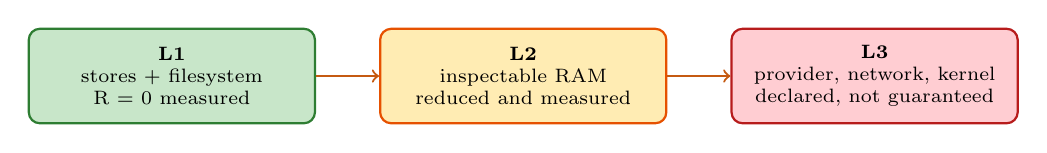
\begin{tikzpicture}[font=\scriptsize,
  tappa/.style={rectangle, draw, rounded corners, align=center, text width=3.4cm, minimum height=1.2cm}]
\node[tappa, fill=palegreen, draw=okgreen, thick] (l1) {\textbf{L1} \\ stores + filesystem \\ R = 0 measured};
\node[tappa, fill=paleamber, draw=warngold, thick, right=0.8cm of l1] (l2) {\textbf{L2} \\ inspectable RAM \\ reduced and measured};
\node[tappa, fill=palered, draw=riskred, thick, right=0.8cm of l2] (l3) {\textbf{L3} \\ provider, network, kernel \\ declared, not guaranteed};
\draw[->, thick, ghostaccent] (l1) -- (l2);
\draw[->, thick, ghostaccent] (l2) -- (l3);
\end{tikzpicture}
\caption{The three disappearance levels. Only L1 is a guarantee; L2 is a measurement; L3 is a declared limit.}
\end{figure}

On 43 bits --- 13 digits --- verifiable and non-invertible are mutually exclusive:
if the commitment is verifiable, anyone can enumerate $10^{13}$ candidates and open
it. v0.02 takes both exits: it raises entropy to 19 digits and declares window T.

\section{v0.02 architecture: what actually changes}
\texttt{src/fantasma}: \texttt{secret.py} (\texttt{SecretBytes} in wipeable bytearray,
\texttt{OneTimeKey}, \texttt{SecretRegion} with construction-time wipe even on
exception), \texttt{crypto.py} (stdlib encrypt-then-MAC over bytearray, scrypt,
\texttt{TimedCommitment}), \texttt{ghost\_window.py} (guard rail against accidental
fork, traceback release), \texttt{hygiene.py} (punctual mlock on the region, never
mlockall), \texttt{forensics.py} (runtime canaries, 7 encodings, store and filesystem
scan, R as unexpected copies, conditional claim), \texttt{pipeline\_v02.py} (same
\texttt{.process()} interface, new interior), \texttt{bench\_gsm8k.py} (GSM8K harness).

\begin{figure}[h]
\centering
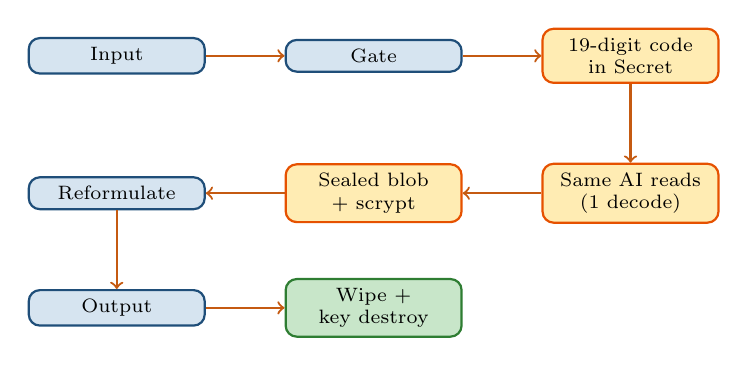
\begin{tikzpicture}[node distance=1.0cm, auto,
  blocco/.style={rectangle, draw=ghostblue, fill=paleblue, thick, rounded corners, text width=2.0cm, align=center, font=\scriptsize},
  evoca/.style={rectangle, draw=warngold, fill=paleamber, thick, rounded corners, text width=2.0cm, align=center, font=\scriptsize},
  chiude/.style={rectangle, draw=okgreen, fill=palegreen, thick, rounded corners, text width=2.0cm, align=center, font=\scriptsize},
  freccia/.style={->, thick, ghostaccent}]
\node[blocco] (in) {Input};
\node[blocco, right=of in] (gate) {Gate};
\node[evoca, right=of gate] (ghost) {19-digit code in Secret};
\node[evoca, below=of ghost] (interp) {Same AI reads (1 decode)};
\node[evoca, left=of interp] (seal) {Sealed blob + scrypt};
\node[blocco, left=of seal] (ref) {Reformulate};
\node[blocco, below=of ref] (out) {Output};
\node[chiude, right=of out] (amn) {Wipe + key destroy};
\draw[freccia] (in) -- (gate);
\draw[freccia] (gate) -- (ghost);
\draw[freccia] (ghost) -- (interp);
\draw[freccia] (interp) -- (seal);
\draw[freccia] (seal) -- (ref);
\draw[freccia] (ref) -- (out);
\draw[freccia] (out) -- (amn);
\end{tikzpicture}
\caption{v0.02 cycle. The cache holds only undecipherable blobs; the key dies by memset.}
\end{figure}

\textbf{Canonical 19-digit code (63.1 bits), never an integer.} The leading zero is
significant; numeric serializations are caught by the scanner's \texttt{int-decimal}
and \texttt{int-hex} variants.

\textbf{Measured scrypt, not hoped.} N$=2^{14}$, r$=8$, p$=1$: steady-state median
$\sim$44~ms per guess on one core, $\sim$14,000 core-years over $10^{13}$.
But scrypt is bandwidth-bound: on 1 GPU $\sim$3.2 years for 13 digits, on 100 GPUs
$\sim$12 days. At 19 digits: millions of years even on GPUs. The per-core number is
not the defense; entropy is.

\begin{figure}[h]
\centering
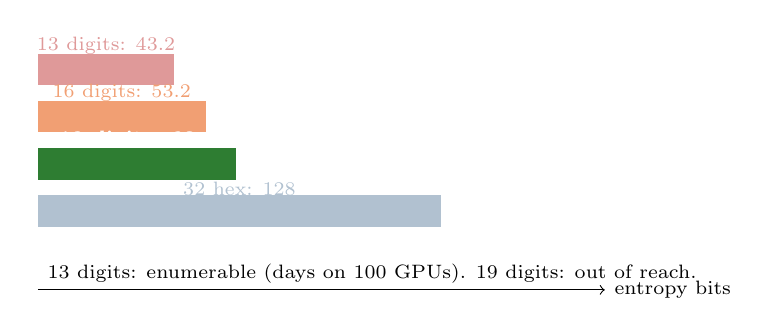
\begin{tikzpicture}[font=\scriptsize]
\draw[->] (0,0) -- (7.2,0) node[right] {entropy bits};
\fill[riskred!45] (0,2.6) rectangle (1.73,3.0) node[midway, above=2pt] {13 digits: 43.2};
\fill[warngold!55] (0,2.0) rectangle (2.13,2.4) node[midway, above=2pt] {16 digits: 53.2};
\fill[okgreen] (0,1.4) rectangle (2.52,1.8) node[midway, above=2pt, white] {\textbf{19 digits: 63.1}};
\fill[ghostblue!35] (0,0.8) rectangle (5.12,1.2) node[midway, above=2pt] {32 hex: 128};
\node[anchor=west] at (0,0.2) {13 digits: enumerable (days on 100 GPUs). 19 digits: out of reach.};
\end{tikzpicture}
\caption{The real lever is entropy, not the KDF. At 43 bits, verifiable and secret exclude each other.}
\end{figure}

\textbf{Declared time window.} Within T the commitment verifies via a live-window
keyed tag; after \texttt{expire()} only one-way scrypt remains. It is the Vision's
``time limits'' item applied to the audit: verifiable within T, one-way after T.

\textbf{Wipe by construction.} \texttt{SecretRegion} memsets via ctypes in
\texttt{\_\_exit\_\_} always, even on early return or exception. Measured: a retained
reference plus early return still yield a zeroed buffer. \texttt{expose\_mutable()}
remains a low-level API; the pipeline goes through the manager.

\textbf{Punctual hygiene.} No mlockall: only mlock on the secret region with a
per-page report. The report says ``designated region protected'', never ``nothing
in swap'': copies outside the region are not locked. The L2 claim requires a
successful lock plus core dumps off plus a zero scan, otherwise it is not made.

\section{Conditional claim: guarantee versus evidence}
A guarantee is a sentence with a guard in front. \texttt{evaluate\_claim()}:
L1 always claimable on its own stores; L2 only with green hygiene and a clean scan;
L3 never. R $=$ found copies minus declared legitimate copies: the scanner holds
the canary to search for it, so that copy is subtracted, otherwise R measures itself.
Mandatory positive and negative controls on every run: without a positive that finds
the injected leak, R$=$0 means nothing. ``Not found'' holds only for the seven
searched encodings: raw, UTF-16LE/BE, hex, base64, int-decimal, int-hex.

\begin{figure}[h]
\centering
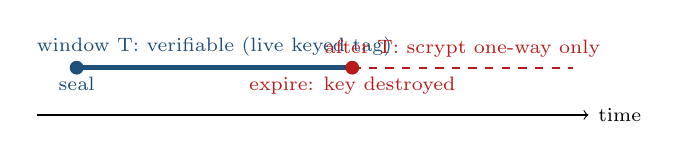
\begin{tikzpicture}[font=\scriptsize]
\draw[->] (0,0) -- (7,0) node[right] {time};
\draw[ghostblue, ultra thick] (0.5,0.6) -- (4.0,0.6) node[midway, above] {window T: verifiable (live keyed tag)};
\fill[ghostblue] (0.5,0.6) circle (2.5pt) node[below] {seal};
\fill[riskred] (4.0,0.6) circle (2.5pt) node[below] {expire: key destroyed};
\draw[riskred, thick, dashed] (4.0,0.6) -- (6.8,0.6) node[midway, above] {after T: scrypt one-way only};
\end{tikzpicture}
\caption{The paradox resolved instead of dodged: verifiable within T, one-way after T.}
\end{figure}

\section{Measured limits, not hidden ones}
\texttt{bytes} cannot be overwritten, \texttt{bytearray} can: the key lives in a
mutable buffer, dropping the reference is hygiene, not erasure. \texttt{del} and
\texttt{gc} free without overwriting: zero L1 holds for the stores, not for RAM.
\texttt{f\_locals} scrubbing is write-through only since Python 3.13 and only on
live frames: on traceback-suspended frames the write does not propagate (measured,
verified zero); the robust path stays \texttt{finally} plus traceback release.
\texttt{ghost\_window} prevents accidental fork from Python code, it is not a barrier
against subprocess or C extensions; on Windows fork does not exist and the start
method is spawn. AES-GCM via OpenSSL copies the plaintext in C: for a disappearance
claim in-place stdlib is architecturally better, with AEAD migration still planned
for v1.0. On Windows without \texttt{/proc} and without mlock, L2 is unmeasurable
and unclaimed: that is the guard working, not a failure.

Docker measurement (Linux 6.6 WSL2, Python 3.11.17, green hygiene, lock on 19 bytes),
19-digit canary, memory regions containing the canary:

\begin{figure}[h]
\centering
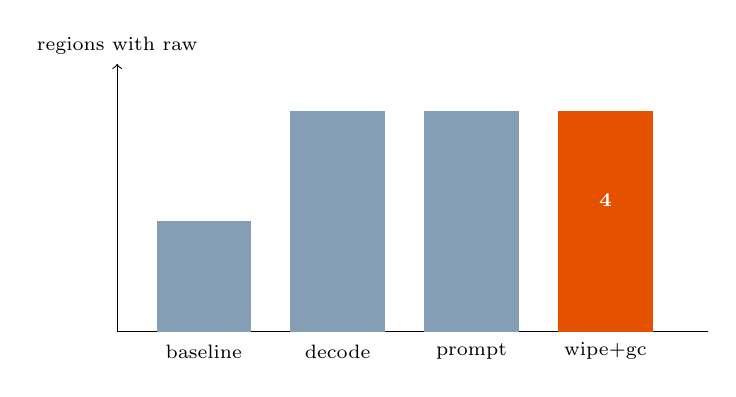
\begin{tikzpicture}[font=\scriptsize]
\draw[->] (0,0) -- (0,3.4) node[above] {regions with raw};
\draw (0,0) -- (7.5,0);
\fill[ghostblue!55] (0.5,0) rectangle (1.7,1.4) node[midway, above=2pt] {2};
\node at (1.1,-0.25) {baseline};
\fill[ghostblue!55] (2.2,0) rectangle (3.4,2.8) node[midway, above=2pt] {4};
\node at (2.8,-0.25) {decode};
\fill[ghostblue!55] (3.9,0) rectangle (5.1,2.8) node[midway, above=2pt] {4};
\node at (4.5,-0.25) {prompt};
\fill[warngold] (5.6,0) rectangle (6.8,2.8) node[midway, above=2pt, white] {\textbf{4}};
\node at (6.2,-0.25) {wipe+gc};
\end{tikzpicture}
\caption{L2 does not return to zero: baseline 2, after decode 4, after wipe and gc still 4. Reduced and measured.}
\end{figure}

\section{Evidence: GSM8K at 50}
Harness in \texttt{src/fantasma/bench\_gsm8k.py}: 50 test-split problems, fixed seed
20261010, three arms on the same DeepSeek-V4.1-Flash with the same final
\texttt{\#\#\#\# number} format. Results in \texttt{outputs/benchmark/}.

\begin{center}
\begin{tabular}{lccc}
\rowcolor{ghostblue}\textcolor{white}{Arm} & \textcolor{white}{Accuracy} & \textcolor{white}{Mean time} & \textcolor{white}{Notes} \\
\midrule
Direct & 46/50 = 0.920 & 2.6 s & one call \\
Hidden CoT & 46/50 = 0.920 & 2.8 s & one call \\
\rowcolor{palegreen}\textbf{Ghost v0.02} & \textbf{47/50 = 0.940} & 10.7 s & two calls + seal \\
\bottomrule
\end{tabular}
\end{center}

\begin{figure}[h]
\centering
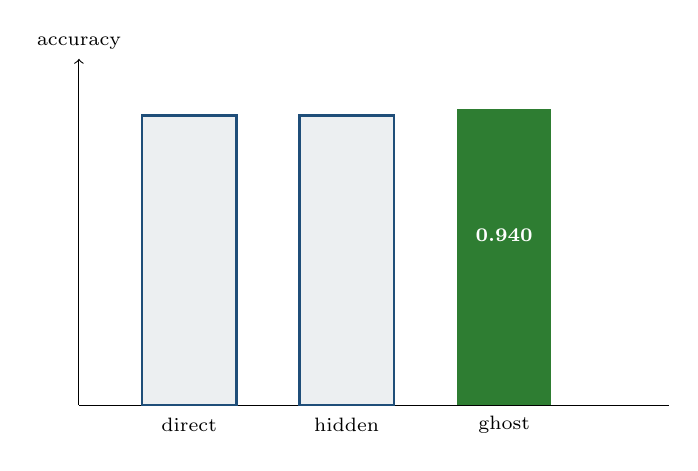
\begin{tikzpicture}[font=\scriptsize]
\draw[->] (0,0) -- (0,4.4) node[above] {accuracy};
\draw (0,0) -- (7.5,0);
\fill[palegray] (0.8,0) rectangle (2.0,3.68) node[midway, above=2pt] {0.920};
\draw[ghostblue, thick] (0.8,0) rectangle (2.0,3.68);
\node at (1.4,-0.25) {direct};
\fill[palegray] (2.8,0) rectangle (4.0,3.68) node[midway, above=2pt] {0.920};
\draw[ghostblue, thick] (2.8,0) rectangle (4.0,3.68);
\node at (3.4,-0.25) {hidden};
\fill[okgreen] (4.8,0) rectangle (6.0,3.76) node[midway, above=2pt, white] {\textbf{0.940}};
\node at (5.4,-0.25) {ghost};
\end{tikzpicture}
\caption{GSM8K at 50: one notch above, same model. A pilot, not a proof.}
\end{figure}

Guarantee side on the ghost cycle: ghost active 48/50 (2 legitimate standbys),
audit verified 50/50, memory and cache empty 50/50, valid format throughout.
A single problem separates the arms --- gold 54, ghost right, the others wrong
together at 27 --- and there is no case where the ghost fails alone. With a model
already at 92\% the signal is weak by construction: we declare it a pilot.

\section{What changes since v0.01}
Caesar $\to$ stdlib shredding; naked HMAC $\to$ scrypt; 13 digits $\to$ canonical 19;
reference drop $\to$ construction-time memset; mlockall $\to$ punctual mlock;
``it disappears'' $\to$ L1/L2/L3 with guards; windowless audit $\to$ window T;
12 tests $\to$ 44 tests; no benchmark $\to$ GSM8K at 50 with three arms.

\begin{figure}[h]
\centering
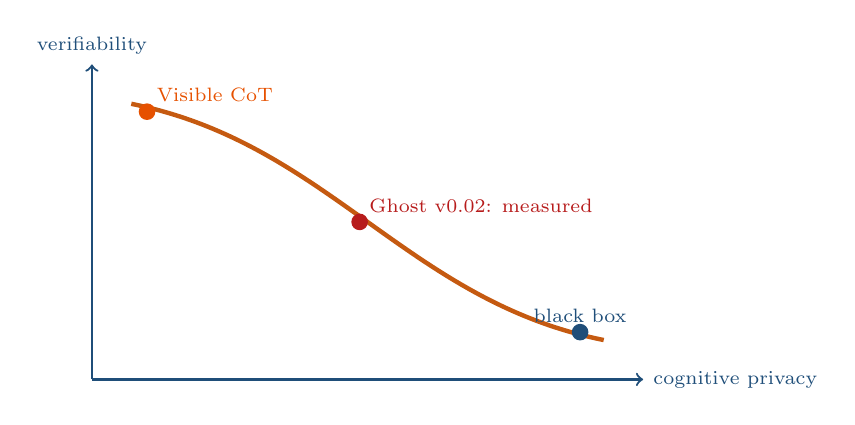
\begin{tikzpicture}[font=\scriptsize]
\draw[->, ghostblue, thick] (0,0) -- (7,0) node[right] {cognitive privacy};
\draw[->, ghostblue, thick] (0,0) -- (0,4) node[above] {verifiability};
\draw[ghostaccent, ultra thick] (0.5,3.5) .. controls (3,3) and (4,1) .. (6.5,0.5);
\fill[warngold] (0.7,3.4) circle (3pt) node[above right] {Visible CoT};
\fill[riskred] (3.4,2.0) circle (3pt) node[above right] {Ghost v0.02: measured};
\fill[ghostblue] (6.2,0.6) circle (3pt) node[above] {black box};
\end{tikzpicture}
\caption{Same curve as v0.01, but the Ghost's point now has measured coordinates.}
\end{figure}

\section{Toward v0.03: the prepared ground}
The question stands unanswered since the first note: does the Ghost actually improve
answers over hidden CoT? The ground is ready: three-arm harness, fixed seeds,
validated format. v0.03 scales to 200 problems with stratified sampling on cases
where direct fails, adds statistical significance, tries the local open-weights
model where L3 narrows, and introduces independent gate supervision with selective
reset. The rest --- supervision, extended time limits, the local/remote split ---
is the v1.0 roadmap.

\begin{figure}[h]
\centering
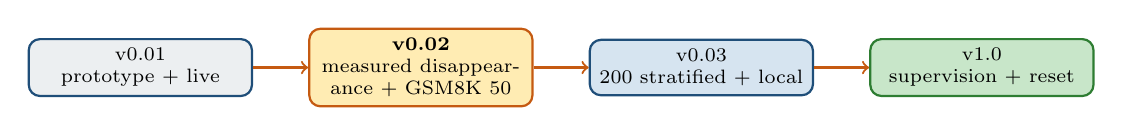
\begin{tikzpicture}[font=\scriptsize,
  tappa/.style={rectangle, draw=ghostblue, thick, rounded corners, align=center, text width=2.6cm}]
\node[tappa, fill=palegray] (v1) {v0.01 \\ prototype + live};
\node[tappa, fill=paleamber, draw=ghostaccent, right=0.7cm of v1] (v2) {\textbf{v0.02} \\ measured disappearance + GSM8K 50};
\node[tappa, fill=paleblue, right=0.7cm of v2] (v3) {v0.03 \\ 200 stratified + local};
\node[tappa, fill=palegreen, draw=okgreen, right=0.7cm of v3] (v4) {v1.0 \\ supervision + reset};
\draw[->, thick, ghostaccent] (v1) -- (v2);
\draw[->, thick, ghostaccent] (v2) -- (v3);
\draw[->, thick, ghostaccent] (v3) -- (v4);
\end{tikzpicture}
\caption{Updated roadmap: measurement exists, now significance.}
\end{figure}

\section{Status and reproducibility}
44 green tests (\texttt{pytest tests/}), 12 originals intact. L2 measurements on
Linux 6.6 WSL2, Python 3.11.17, Docker with memlock unlocked; application
measurements on Windows 10.0.26200, Python 3.13.13. Dataset \texttt{openai/gsm8k}
test split, seed 20261010, model \texttt{deepseek-flash} with
\texttt{reasoning\_effort=high}. Key from env only, never in code. Otherwise it
stays in the notebook: this one, for now, measures instead of promising.
\end{document}
